%%%%%%%%%%%%%%%%%%%%%%%%%%%%%%%%%%%%%%%%%%%%%%%%%%%%%
%												    %
%	REDES DE COMPUTADORES						 %
%												    %
%	Novembro 2015								    %
%												    %
%	Angela Cardodo e Bruno Madeira					%
%   											    %	
%%%%%%%%%%%%%%%%%%%%%%%%%%%%%%%%%%%%%%%%%%%%%%%%%%%%%

\documentclass[11pt,a4paper,reqno]{report}
\linespread{1.2}


\usepackage{rotating}
\usepackage{tikz}
\usepackage[active]{srcltx}    
\usepackage{graphicx}
\usepackage{amsthm,amsfonts,amsmath,amssymb,indentfirst,mathrsfs,amscd}
\usepackage[mathscr]{eucal}
\usepackage{tensor}
%\usepackage[utf8x]{inputenc}

\usepackage[utf8]{inputenc}

\usepackage[portuges]{babel}
\usepackage[T1]{fontenc}
\usepackage{enumitem}
\setlist{nolistsep}
\usepackage{comment} 
\usepackage{tikz}
\usepackage[numbers,square, comma, sort&compress]{natbib}
\usepackage[nottoc,numbib]{tocbibind}
%\numberwithin{figure}{section}
\numberwithin{equation}{section}
\usepackage{scalefnt}
\usepackage[top=1cm, bottom=2cm, left=2cm, right=2cm]{geometry}
%\usepackage{tweaklist}
%\renewcommand{\itemhook}{\setlength{\topsep}{0pt}%
%	\setlength{\itemsep}{0pt}}
%\renewcommand{\enumhook}{\setlength{\topsep}{0pt}%
%	\setlength{\itemsep}{0pt}}
%\usepackage[colorlinks]{hyperref}
\usepackage{MnSymbol}
%\usepackage[pdfpagelabels,pagebackref,hypertexnames=true,plainpages=false,naturalnames]{hyperref}
\usepackage[naturalnames]{hyperref}
\usepackage{enumitem}
\usepackage{titling}
\newcommand{\subtitle}[1]{%
	\posttitle{%
	\par\end{center}
	\begin{center}\large#1\end{center}
	\vskip0.5em}%
}
\newcommand{\HRule}{\rule{\linewidth}{0.5mm}}
\usepackage{caption}
\usepackage{etoolbox}% http://ctan.org/pkg/etoolbox
\usepackage{complexity}

\usepackage[official]{eurosym}

\def\Cpp{C\raisebox{0.5ex}{\tiny\textbf{++}}}

\makeatletter
\def\@makechapterhead#1{%
  %%%%\vspace*{50\p@}% %%% removed!
  {\parindent \z@ \raggedright \normalfont
    \ifnum \c@secnumdepth >\m@ne
        \huge\bfseries \@chapapp\space \thechapter
        \par\nobreak
        \vskip 20\p@
    \fi
    \interlinepenalty\@M
    \Huge \bfseries #1\par\nobreak
    \vskip 40\p@
  }}
\def\@makeschapterhead#1{%
  %%%%%\vspace*{50\p@}% %%% removed!
  {\parindent \z@ \raggedright
    \normalfont
    \interlinepenalty\@M
    \Huge \bfseries  #1\par\nobreak
    \vskip 40\p@
  }}
\makeatother

\usepackage[toc,page]{appendix}

\addto\captionsportuges{%
  \renewcommand\appendixname{Anexo}
  \renewcommand\appendixpagename{Anexos}
}

\addto\captionsportuges{%
  \renewcommand\abstractname{\huge Sumário}  
}

\usepackage{verbatim}
\usepackage{color}
\definecolor{darkgray}{rgb}{0.41, 0.41, 0.41}
\definecolor{green}{rgb}{0.0, 0.5, 0.0}
\usepackage{listings}
\lstset{language=C++, 
    basicstyle=\linespread{0.8}\ttfamily,
    keywordstyle=\color{blue}\ttfamily,
	showstringspaces=false,
    stringstyle=\color{red}\ttfamily,
    commentstyle=\color{green}\ttfamily,
	identifierstyle=\color{darkgray}\ttfamily,
    morecomment=[l][\color{magenta}]{\#},
	tabsize=4,
    breaklines=true
}

\begin{document}



\begin{titlepage}
\begin{center}
 
\vspace*{3cm}

{\Large Redes de Computadores}\\[2cm]

% Title
{\Huge \bfseries Protocolo de Liga\c{c}\~ao de Dados \\[1cm]}

% Author
{\large \^Angela Cardoso e Bruno Madeira}\\[2cm]


\includegraphics[width=10cm]{feup_logo.jpg}\\[2cm]


% Bottom of the page
{\large \today}

\end{center}
\end{titlepage}


%%%%%%%%%%%
% SUMARIO %
%%%%%%%%%%%
\begin{abstract}
	
Este relatório tem como objectivo reportar o segundo trabalho prático relativo a Redes de Computadores da Licenciatura com Mestrado em Engenharia Informátia e Computação. 


\end{abstract}

\tableofcontents

%%%%%%%%%%%%%%
% INTRODUCAO %
%%%%%%%%%%%%%%
\chapter{Introdução}


	
%%%%%%%%%%%%%%%
% APLICAÇÂO %
%%%%%%%%%%%%%%%
\chapter{Aplicação}

A aplicação desenvolvida realiza o download de um ficheiro fazendo uso do protocolo FTP segundo o  \href{https://www.ietf.org/rfc/rfc959.txt}{RFC959}.
Para tal são usadas duas sockets, uma para comandos e outra para dados, de acordo com o modelo descrito na secção 2.3 do RFC959.
Os comandos usados podem ser verificados na secção 4 (páginas 25 a 34) do RFC959 e na página 47. É usado o comando PASV sendo que o servidor não usa a porta default para os dados (porta 20) e fica à espera que o cliente estabeleça a ligação.

Todas as funcionalidades desenvolvidas ligadas ao protocolo FTP podem ser verificadas no ficheiro ftp.c e ftp.h dispoíveis nos anexos ~\ref{FTPC} e ~\ref{FTPH}. Apesar de existir uma função denominada ftp\_abort esta não envia um comando ABORT (embora esta tenha sido a funcionalidade inicialmente pensada para o mesmo). Esta função apenas fecha as sockets em caso de erro.\\

Para efectuar ligação ao servidor a aplicação deve também receber um URL no formato estabelecido no  \href{https://www.ietf.org/rfc/rfc1738.txt}{RFC1738}. Não consideramos utilizadores anónimos como é referido na secção 3.2.1. do RFC1738. No downloader.c (ver anexo ~\ref{DOWNLOADERC}) é realizado o parsing do url ficando guardado numa estrutura o nome de utilizador, password, nome do host, caminho até ao ficheiro e o nome do ficheiro.

Uma vez realizado o parsing tenta-se obter o ip do destino e cria-se uma ligação TCP para a porta 21 do servidor a fim de enviar os comandos para pedir a recepção do ficheiro. As funções usadas para obter o ip e para estabelecer são as disponibilizadas nos exemplos do moodle da disciplina. A conexão é realizada com a função connect e não o bind uma vez que a aplicação está do lado do cliente. É utilizada a função gethostbyname para obter o ip, que funciona mas está depreciada segundo o \href{ http://beej.us/guide/bgnet/output/html/multipage/index.html}{Beej's Guide to Network Programming}.\\

Em termos de estrutura foram desenvolvidos apenas 4 modulos que apresentamos seguidamente.
\begin{itemize} 
\item downloader - Onde se encontra a função main da aplicação. Também é responsável pelo parsing e por obter o ip destino.
\item ftp -  Implementa e disponibiliza comandos do protocolo ftp. Os file descriptors das sockets também se encontram neste módulo.
\item socket - Apenas disponibiliza uma função para conectar sockets.
\item utilities - Apenas disponibiliza auxiliares para debug.
\end{itemize}

%%%%%%%%%%%%%%%%%%%%
% LABS REALIZADOS%
%%%%%%%%%%%%%%%%%%%%
\chapter{Experiências}

\section{Experiência 1 - Configurar uma Rede IP}

Nesta experiência criou-se uma LAN com o tux1 e o tux4 na mesma rede e configurados os seus endereços ip. Usando o comando ping na etapa 7, pudemos verificar o envio de um comando ARP em broadcast pelo tux1 que procurava o endereço físico do tux4, necessário ao protocolo ethernet usado para poder comunicar dentro de uma mesma rede local. Seguidamente vericou-se a resposta do tux4 e foi realizado o ping com sucesso.

Atentando nos pacotes capturados com o wireshark do anexo~\ref{ex1_headers} é possível verificar que os pacotes ARP são identificáveis pelo cabeçalho Ethernet x0806 e os IP pelo x0800. As mensagens de ping podem ser identificadas pelo cabeçalho Ethernet correspondente ao protocolo IP e pelo cabeçalho de IP x01 que corresponde ao protocolo ICMP.

...\\ TODO frame length \\

Na lista de pacotes recebidos existe também pacotes do tipo loopback. Este são pacotes que são redireccionados para a máquina que os emitiu com a finalidade (tipicamente) de verificar se esta se encontra em estado operacional. Neste caso, os pacotes recebidos aparentam ser do switch, tendo como endereço de origem e destino o CiscoInc\_3a:f1:03.

\section{Experiência 2 - Implementar 2 LANs num switch}

Foram criadas duas LANs uma com o tux1 e o tux4 na rede 172.16.60.0 outra com o tux2 na 172.16.61.0 (com máscara de 24 bits) atribuindoendereços  ip às máquinas relativos à rede em que se deviam encontrar e configurando o switch de modo a funcionarem como 2 redes distintas. Constatou-se que apenas  computadores que se encontravam na mesma rede virtual local podiam comunicar entre si. Nos anexos ~\ref{ex2_tux1ping_tux2} e ~\ref{ex2_tux1ping_tux4} verifica-se que pings realizados do tux1 em broadcast (alignea 7 do trabalho prático) chegam ao tux4 mas não ao tux2. Similarmente, não foi possível encontrar pacotes de ICMP no tux1 e no tux4 quando realizado ping apartir do tux2 como se pode observar nos anexos seguintes.


\section{Experiência 3 - Configurar um Router em Linux}
...
\section{Experiência 4 - Configurar um Router Comercial e Implementar NAT}
...
\section{Experiência 5 - DNS}

\section{Experiência 6 - Conexões TCP}

Nesta experiência usámos a aplicação desenvolvida para realizar o download de um ficheiro. Foi chamada a aplicação inicialmente no TUX1 e seguidamente após um pequeno intervalo de tempo no TUX2. Parte do download no TUX2 foi realizado em simutâneo do realizado no TUX1.\\

Como esperado, devido ao protocolo FTP, pudemos verificar o \emph{3-way handshake} de duas conexões TCP. O primeiro relativo à ligação usada para envio de comandos e o segundo relativo a de envio de dados que podem ser verificados no anexo ~\ref{ex6_tux1_handshakes}. O estabelecimento de conexão consiste no pedido do cliente ao servidor para estabelecer ligação (SYN) seguido da resposta do servidor (SYN,ACK) e de uma confirmação final pelo cliente (ACK) que podem ser melhor observados no anexo ~\ref{ex6_tux1_1sthandshake} onde é mostrado também o número de sequência e de confirmação em cada pacote.\\

O mecanismo de ARQ (Automatic Repeat Request) do protocolo TCP é uma variante do Go-Back-N onde o servidor envia confirmações relativas a cada segmento que recebe. 

Perto de quando o TUX1 atinge o seu plateu máximo de tráfego, aos 14 segundos d gráfico ~\ref{ex6_a5_1io}, podem ser observadas vários pacotes do tipo [duplicate ACK], [Previous Segment not captured],[Fast Retransmission] e [Retransmission] que parecem indicar congestionamento.
Segundo o \href{http://www.ietf.org/rfc/rfc2581.txt}{RFC2581} o receptor deve enviar um duplicate ACK quando é recebido um segmento fora de ordem e pode ocorrer uma retransmissão, \emph{fast retransmit}, após a recepção de 3 confirmações duplicadas (duplicate ACKs) pelo transmissor. Na experiência foram capturados pelo Wireshark pacotes que parecem demonstrar este comportamento como se pode pelo anexo ~\ref{ex6_retrans}.\\


TODO...\\

Na realização da última alínea pudemos verificar que a recepção de dados quando usada uma segunda ligação no TUX2 era afectada. Pode observar-se nos anexos ~\ref{ex6_a5_1io} e ~\ref{ex6_a5_2io} que a recepção  tende para um plateu máximo no TUX1 que é quebrado devido à ligação estabelecida pelo TUX2. Observando o gráfico relativo ao TUX2 podemos ver que este atinge um plateu máximo perto do final da sua ligação que ocorre devido ao TUX1 já ter terminado o download. Além deste plateu máximo podemos verificar que os gráficos são complementares no sentido em que a soma das funções dos dois gráficos, alinhando-os consoante os seus pontos mínimos e máximos dado que as leituras em wireshark não foram iniciadas em simultâneo, resulta aproximadamente numa função constante que apresenta uma recepção entre 10000 e 12000 packets por segundo.

\section{Experiência 7 - Implementar NAT em Linux}

%%%%%%%%%%%%%%
% CONCLUSOES %
%%%%%%%%%%%%%%
\chapter{Conclusões}

%%%%%%%%%%%%%%
% NOTAS IMPORTANTES %
%%%%%%%%%%%%%%
\chapter{Esclarecimentos}

Apesar de deste relatório referir muitas vezes o TUX2, da experiência 4 até à 7, qualquer referência ao TUX2 corresponde na realidade ao TUX3 uma vez que o TUX2 deixou de estar disponivel apartir de dada altura. Para que o relatório respeite os nomes referidos no guião e usados nos anexos, mantendo a continuidade entre experiências, decidimos continuar a referir-nos ao terceiro computador usado na rede como sendo o TUX2.  

%%%%%%%%%%%%%%%%
% BIBLIOGRAPHY %
%%%%%%%%%%%%%%%%


\begin{appendices}

%%%%%%%%%%%%%%%%%%%%%%%%%%%
% APENDICE - VARIAS %
%%%%%%%%%%%%%%%%%%%%%%%%%%%
\chapter{Enderaços MAC}

\begin{itemize} 
\item TUX1 eth0: 00:0f:fe:8c:af:71
\item TUX2 eth0: 00:21:5a:5a:7d:9c
\item TUX3 eth0: 00:21:5a:61:2f:4e
\item TUX4 eth0: 00:21:5a:c5:61:bb
\item TUX4 eth1: 00:c0:df:04:20:8c
\end{itemize}

\chapter{Console logs}

\section{Ex4 align.4}
\begin{lstlisting}[frame=single]
tux63:~/Desktop/RCOM/scripts# route -n
Kernel IP routing table
Destination     Gateway         Genmask         Flags Metric Ref    Use Iface
0.0.0.0         172.16.61.254   0.0.0.0         UG    0      0        0 eth0
172.16.61.0     172.16.61.254   255.255.255.0   UG    0      0        0 eth0
172.16.61.0     0.0.0.0         255.255.255.0   U     0      0        0 eth0
tux63:~/Desktop/RCOM/scripts# traceroute 172.16.60.1
traceroute to 172.16.60.1 (172.16.60.1), 30 hops max, 60 byte packets
 1  172.16.61.254 (172.16.61.254)  0.498 ms  0.548 ms  0.587 ms
 2  172.16.61.253 (172.16.61.253)  0.873 ms  0.500 ms  0.506 ms
 3  172.16.60.1 (172.16.60.1)  0.799 ms  0.792 ms  0.784 ms
tux63:~/Desktop/RCOM/scripts# ping 172.16.60.1
PING 172.16.60.1 (172.16.60.1) 56(84) bytes of data.
64 bytes from 172.16.60.1: icmp_seq=1 ttl=62 time=0.629 ms
64 bytes from 172.16.60.1: icmp_seq=2 ttl=62 time=0.594 ms
64 bytes from 172.16.60.1: icmp_seq=3 ttl=62 time=0.587 ms
64 bytes from 172.16.60.1: icmp_seq=4 ttl=62 time=0.569 ms
64 bytes from 172.16.60.1: icmp_seq=5 ttl=62 time=0.623 ms
^C
--- 172.16.60.1 ping statistics ---
5 packets transmitted, 5 received, 0% packet loss, time 4000ms
rtt min/avg/max/mdev = 0.569/0.600/0.629/0.031 ms
tux63:~/Desktop/RCOM/scripts# traceroute 172.16.60.1
traceroute to 172.16.60.1 (172.16.60.1), 30 hops max, 60 byte packets
 1  172.16.61.253 (172.16.61.253)  0.465 ms  0.343 ms  0.344 ms
 2  172.16.60.1 (172.16.60.1)  0.666 ms  0.662 ms  0.654 ms
tux63:~/Desktop/RCOM/scripts# route -n
Kernel IP routing table
Destination     Gateway         Genmask         Flags Metric Ref    Use Iface
0.0.0.0         172.16.61.254   0.0.0.0         UG    0      0        0 eth0
172.16.61.0     172.16.61.254   255.255.255.0   UG    0      0        0 eth0
172.16.61.0     0.0.0.0         255.255.255.0   U     0      0        0 eth0
tux63:~/Desktop/RCOM/scripts# 
\end{lstlisting}

\chapter{Wireshark logs and statistics}

\section{Ex1}
\label{ex1_headers}
\subsection{Captura no TUX1 - ARP}
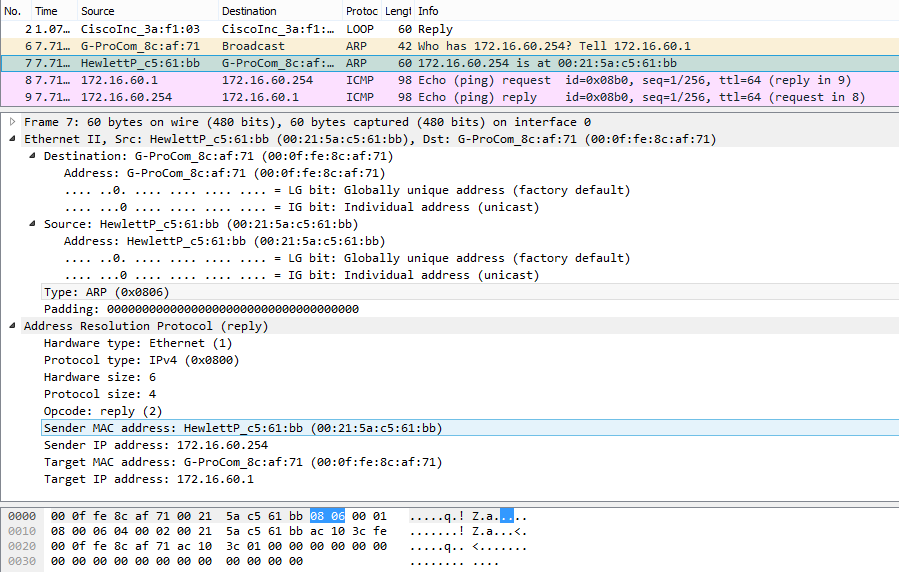
\includegraphics[width=18cm]{ex1_arp.png}
\subsection{Captura no TUX1 - ICMP}
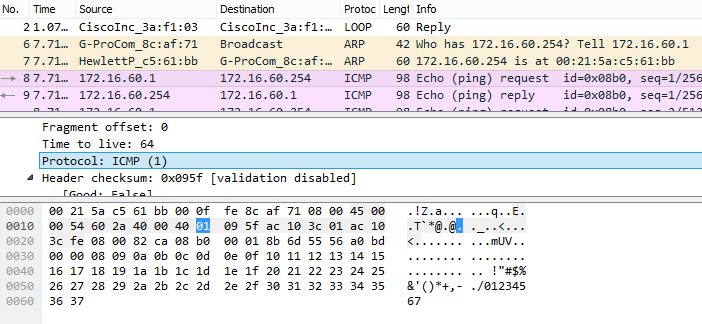
\includegraphics[width=18cm]{ex1_icmp.png}

\section{Ex2}
\subsection{Alínea 7 - Captura no TUX1}
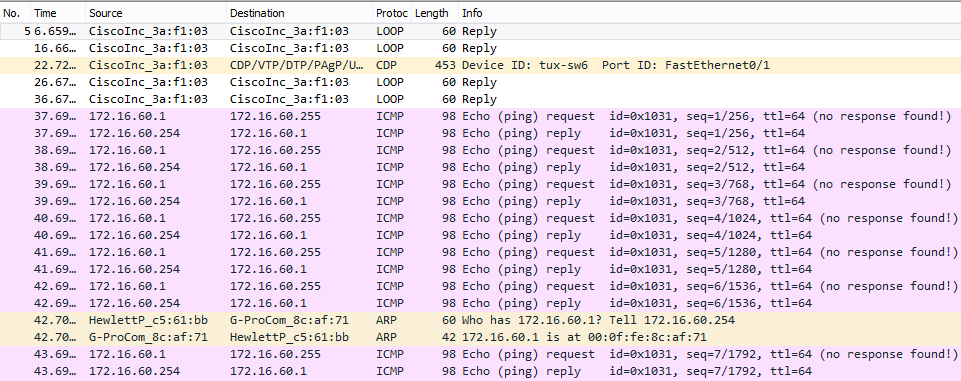
\includegraphics[width=18cm]{ex2_a7_tux1.png}
\subsection{Alínea 7 - Captura no TUX2}
\label{ex2_tux1ping_tux2}
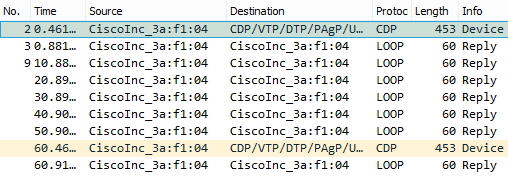
\includegraphics[width=18cm]{ex2_a7_tux2.png}
\subsection{Alínea 7 - Captura no TUX4}
\label{ex2_tux1ping_tux4}
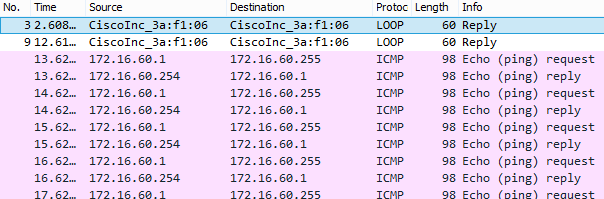
\includegraphics[width=18cm]{ex2_a7_tux4.png}

\subsection{Alínea10 - Captura no TUX1}
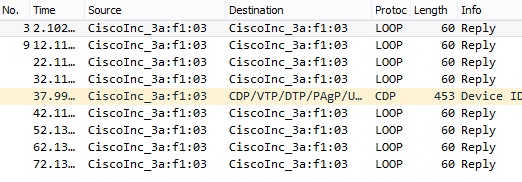
\includegraphics[width=18cm]{ex2_a10_tux1.png}
\subsection{Alínea10 - Captura no TUX2}
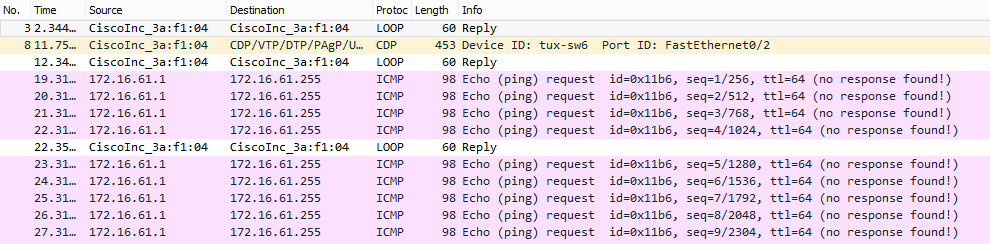
\includegraphics[width=18cm]{ex2_a10_tux2.png}
\subsection{Alínea10 - Captura no TUX4}
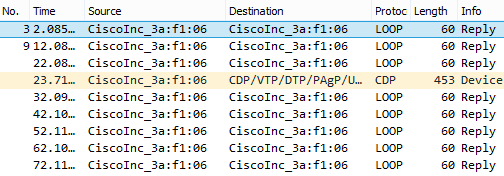
\includegraphics[width=18cm]{ex2_a10_tux4.png}

\section{Ex3}

\section{Ex4}

\section{Ex5}

\section{Ex6}

\subsection{Capturas dos 'hanshakes' no TUX1}
\label{ex6_tux1_handshakes}
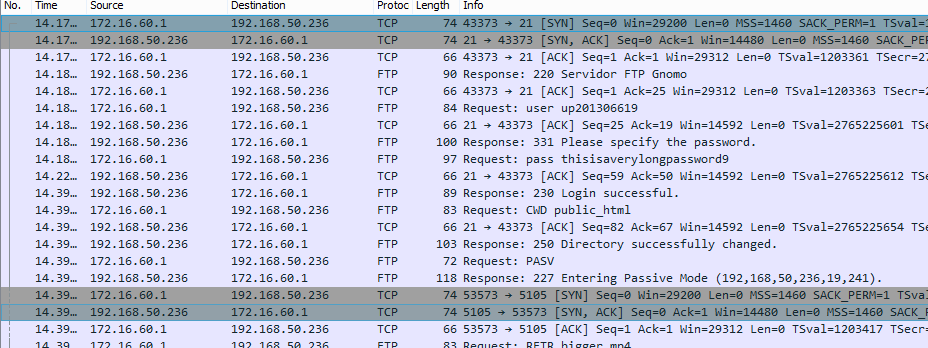
\includegraphics[width=18cm]{ex6_tux1_handshakes.png}

\subsection{Primeiro 'Handshake' no TUX1 em Detalhe}
\label{ex6_tux1_1sthandshake}
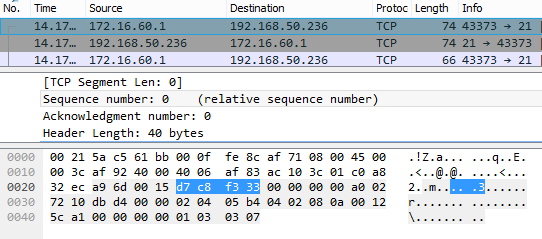
\includegraphics[width=18cm]{ex6_handshake1.png}
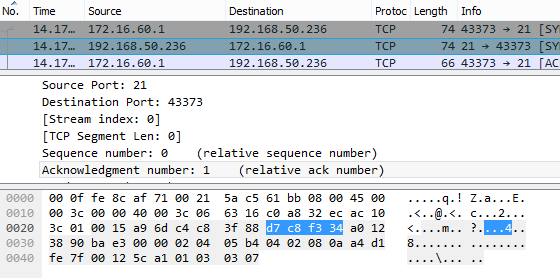
\includegraphics[width=18cm]{ex6_handshake2.png}
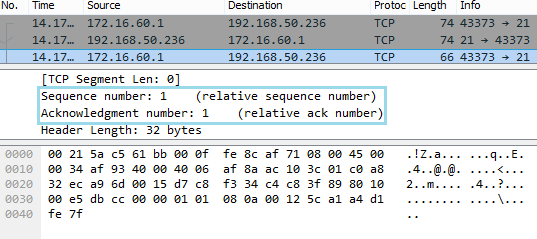
\includegraphics[width=18cm]{ex6_handshake3.png}

\subsection{Capturas no TUX1 de Dup ACK, Fast Retransmission e Retransmission}
\label{ex6_retrans}
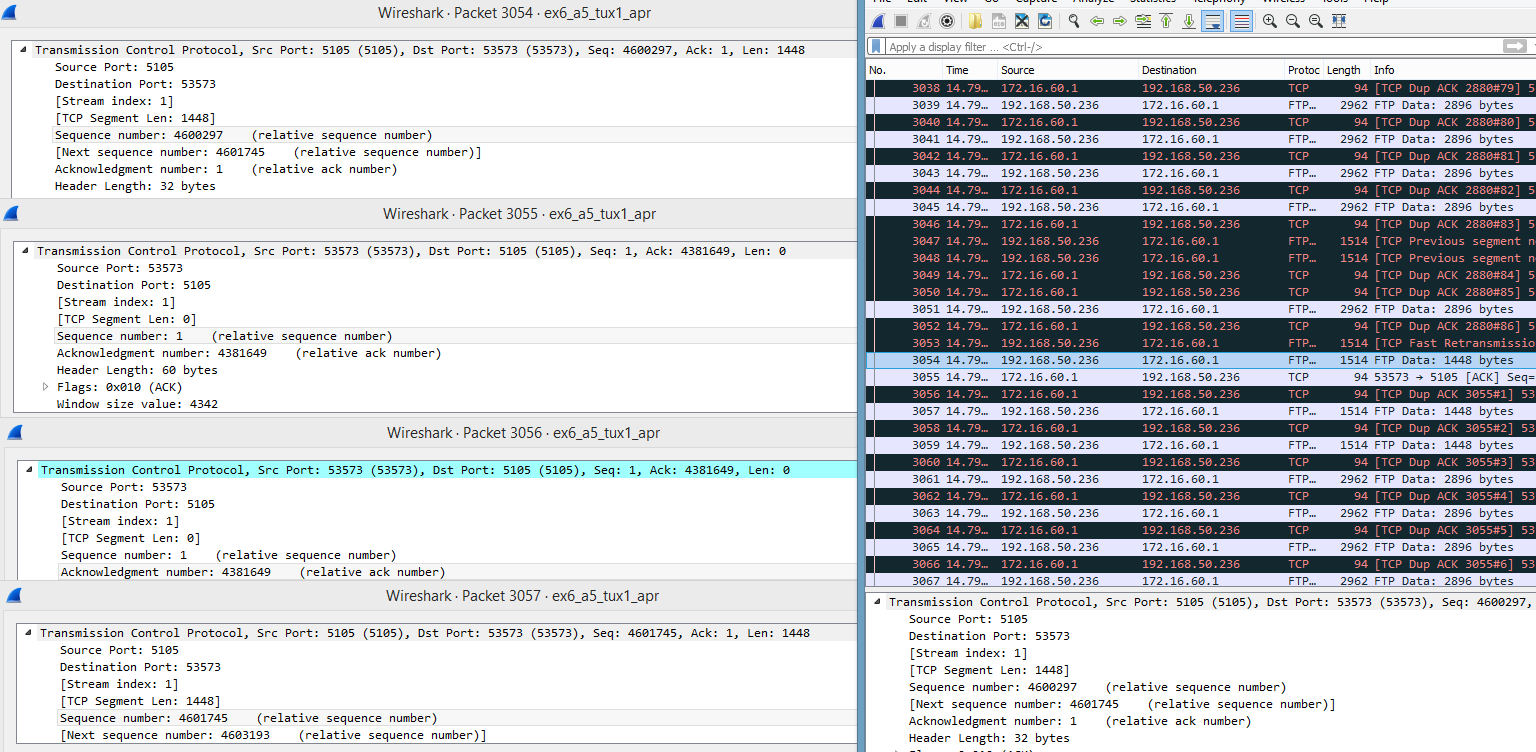
\includegraphics[width=18cm]{ex6_tux1_3054.png}
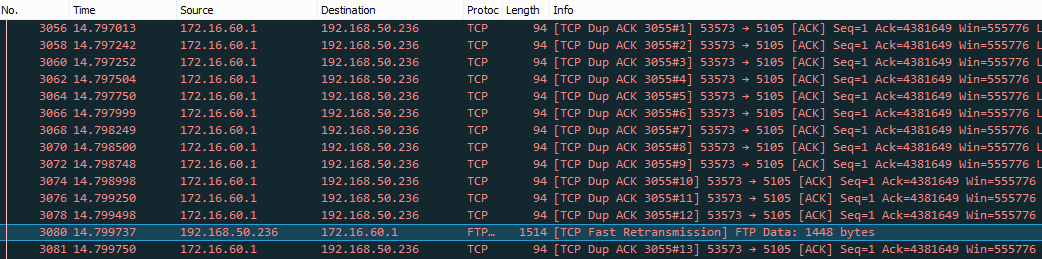
\includegraphics[width=18cm]{ex6_tux1_fastretransmission.png}
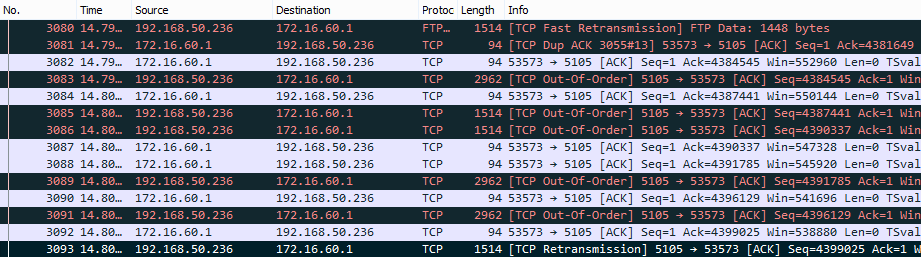
\includegraphics[width=18cm]{ex6_tux1_retransmission.png}

\subsection{Alínea 5 - Gráfico de Tráfego no TUX1}
\label{ex6_a5_1io}
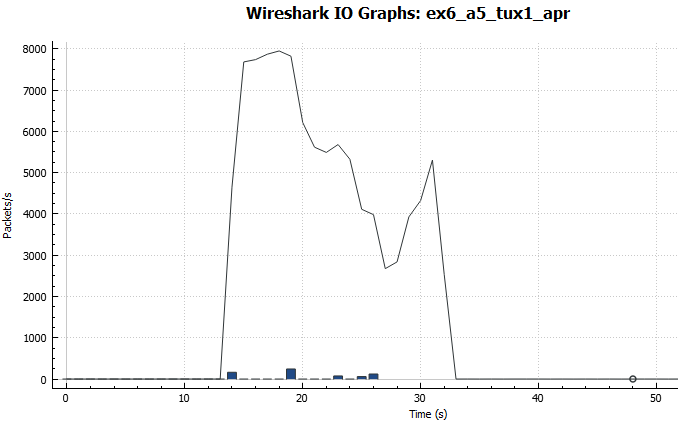
\includegraphics[width=18cm]{ex6_a5_tux1_IO.png}
\subsection{Alínea 5 - Gráfico de Tráfego no TUX2}
\label{ex6_a5_2io}
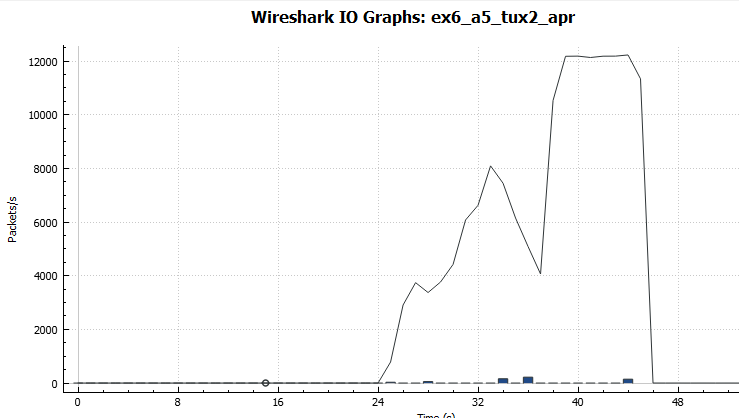
\includegraphics[width=18cm]{ex6_a5_tux2_IO.png}

\section{Ex7}

%%%%%%%%%%%%%%%%%%%%%%%%%%%
% APENDICE - CODIGO FONTE %
%%%%%%%%%%%%%%%%%%%%%%%%%%%
\chapter{Código Fonte}

%%%%%%%%%%%%%%%%%%%%%%%%%%%
\section{downloader.c}
\label{DOWNLOADERC}
%%%%%%%%%%%%%%%%%%%%%%%%%%%

\begin{lstlisting}

#include <string.h>
#include <sys/socket.h>
#include <netinet/in.h>
#include <arpa/inet.h>
#include <netdb.h>
#include <stdlib.h>
#include <unistd.h>
#include <stdio.h>
#include <string.h>
#include <errno.h> 
#include <sys/types.h>
#include "utilities.h"
#include "ftp.h"

//VARS AND STRUCTS --------------------------------------------------------------------------------------
#define FTP_PORT	21
#define MAX_STRING_SIZE 200
struct /*???*/Info{
  char username[MAX_STRING_SIZE];
  char password[MAX_STRING_SIZE];
  char host_name[MAX_STRING_SIZE];
  char url_path[MAX_STRING_SIZE];
  char filename[MAX_STRING_SIZE];
  char ip[MAX_STRING_SIZE];
};

//AUX FUNCS CODE --------------------------------------------------------------------------------------
int parse(char *str, struct Info* info) {
  
  //http://docs.roxen.com/pike/7.0/tutorial/strings/sscanf.xml
	if(4 != sscanf(str, "ftp://[%[^:]:%[^@]@]%[^/]/%s\n", info->username, info->password, info->host_name, info->url_path)) {
		return 1;
	}

  //get filename http://stackoverflow.com/questions/32822988/get-the-last-token-of-a-string-in-c
      char *last = strrchr(info->url_path, '/') ;
      if(last!=NULL) 
      {
	memcpy(info->filename, last+1, strlen(last)+1);
	memset(last,0,strlen(last)+1);
      }
      else {
	strcpy(info->filename,info->url_path);
	memset(info->url_path,0,sizeof(info->url_path));
      }
  
	return 0;
}

int get_ip(struct Info* info) {
	struct hostent* host;

	if ((host = gethostbyname(info->host_name)) == NULL) {
		perror("gethostbyname");
		return 1;
	}

	char* ip = inet_ntoa(*((struct in_addr *)host->h_addr));
	strcpy(info->ip, ip);

	printf("Host name  : %s\n", host->h_name);
	printf("IP Address : %s\n", info->ip);
	
	return 0;
}


//MAIN --------------------------------------------------------------------------------------
#define DEBUG_ALL 1
int main(int argc,char **argv)
{
  struct Info info;
  
  // ftp message composition: ftp://[<user>:<password>@]<host>/<url-path>
  
	// ---- URL stuff ----

	//parse
	if(parse(argv[1],&info)!=OK)
	{
	  printf("\nINVALID ARGUMENT! couldn't be parsed properly.\n");
	  return 1;
	}
	DEBUG_SECTION(DEBUG_ALL,
	printf("\nuser:%s\n",info.username);
	printf("pass:%s\n",info.password);
	printf("host:%s\n",info.host_name);
	printf("urlpath:%s\n",info.url_path);
	printf("filename:%s\n",info.filename);
	);
  
	//- - - - - -
	get_ip(&info);
	
	// ---- FTP stuff -----
		
printf("\n connecting... \n");
	
	if(ftp_connect(info.ip, FTP_PORT)!=OK)
{ftp_abort(); return 1;}

printf("\n logging in... \n");

	if(ftp_login(info.username, info.password)!=OK)// Send user n pass
{ftp_abort(); return 1;}
		

		
	if(strlen(info.url_path)>0) {
	  printf("\n changing dir... \n");
	  
	  if(ftp_changedir(info.url_path)!=OK)// change directory
	  {ftp_abort(); return 1;}
	}
	
printf("\n passive mode... \n");

	if(ftp_pasv()!=OK)// passive mode
{ftp_abort(); return 1;}

printf("\n asking for file... \n");

	if(ftp_retr(info.filename)!=OK)// ask to receive file
{ftp_abort(); return 1;}

printf("\n downloading file... \n");

	if(ftp_download(info.filename)!=OK)// receive file
{ftp_abort(); return 1;}

printf("\n disconecting... \n");

	if(ftp_disconnect()!=OK)// disconnect from server
{ftp_abort(); return 1;}

printf("\n downloader terminated ok! \n");

	return 0;
}

\end{lstlisting}
%%%%%%%%%%%%%%%%%%%%%%%%%%%
\section{Ficheiro ftp.h}
\label{FTPH}
%%%%%%%%%%%%%%%%%%%%%%%%%%%

\begin{lstlisting}

#ifndef FTP
#define FTP

int ftp_connect( const char* ip, int port);
int ftp_disconnect();

int ftp_login( const char* user, const char* password);
int ftp_changedir( const char* path);
int ftp_pasv();
int ftp_retr( const char* filename);
int ftp_download( const char* filename);

void ftp_abort();

#endif

\end{lstlisting}
%%%%%%%%%%%%%%%%%%%%%%%%%%%
\section{Ficheiro ftp.c}
\label{FTPC}
%%%%%%%%%%%%%%%%%%%%%%%%%%%

\begin{lstlisting}

#include <stdio.h>
#include <unistd.h>
#include <string.h>

#include <sys/types.h>
#include <sys/socket.h>


#include "ftp.h"
#include "socket.h"
#include "utilities.h"

#define MAX_STRING_SIZE 500

int control_socket_fd; 
int data_socket_fd;


//------------------------------------------------------------------------
// READ AND SEND
#if 1

int ftp_read(char* str,unsigned long str_total_size)
{
    int bytes = 0;
    if( (bytes = recv(control_socket_fd,str,str_total_size,0)) < 0  )
      {
	perror("ftp_read: recv failed\n");
	return -1;
      }
    return bytes;
}

int ftp_send( const char* str,unsigned long str_size)
{
	    int bytes = 0;
    if( (bytes = send(control_socket_fd,str,str_size,0)) < 0  )
      {
	perror("ftp_read: recv failed\n");
	return -1;
      }
    return bytes;
}

#endif


//------------------------------------------------------------------------
// CONECT AND DISCONECT
#if 1

int ftp_connect( const char* ip, int port) {
	
	int socket_fd;
	char read_bytes[MAX_STRING_SIZE];

	//open control socket
	if ((socket_fd = connect_socket_TCP(ip, port)) < 0)
	{
		printf("ftp_connect: Failed to connect socket\n");
		return 1;
	}

	control_socket_fd = socket_fd;
	data_socket_fd 	  = 0;

	//Try to read with control socket
	if (ftp_read(read_bytes, sizeof(read_bytes))<0)
	{
		printf("ftp_connect: Failed to read\n");
		return 1;
	}

	return 0;
}

int ftp_disconnect() {
	char aux[MAX_STRING_SIZE];

	//read discnnect
		if (ftp_read(aux, sizeof(aux))<0) {
		printf("ftp_disconnect: Failed to disconnect\n");
		return 1;
	}
	//send disconnect 
	sprintf(aux, "QUIT\r\n");
	if (ftp_send(aux, strlen(aux))<0) {
		printf("ftp_disconnect: Failed to output QUIT");
		return 1;
	}
	
	close(control_socket_fd);

	return 0;
}

#endif

//------------------------------------------------------------------------
// MAIN OPERATIONS
#if 1

int ftp_login( const char* user, const char* password) {
	
	char aux[MAX_STRING_SIZE];

	//send username
	sprintf(aux, "user %s\r\n", user);
	if (ftp_send( aux, strlen(aux))< 0) {
		printf("ftp_login: ftp_send failure.\n");
		return 1;
	}
	//receive answer to username
	if (ftp_read( aux, sizeof(aux))<0) {
		printf(	"ftp_login:Bad response to user\n");
		return 1;
	}

	//send password
	memset(aux, 0, sizeof(aux));//reuse 2send
	sprintf(aux, "pass %s\r\n", password);
	if (ftp_send( aux, strlen(aux))< 0) {
		printf("ftp_login: failed to send password.\n");
		return 1;
	}
	//receive answer to password
	if (ftp_read( aux, sizeof(aux))<0) 
	{
		printf(	"ftp_login:Bad response to pass\n");
		return 1;
	}

	return 0;
}

int ftp_changedir(const char* path) {
	
	char aux[MAX_STRING_SIZE];

	//send cwd command
	sprintf(aux, "CWD %s\r\n", path);
	if (ftp_send(aux, strlen(aux))< 0) {
		printf("ftp_changedir:Failed to send\n");
		return 1;
	}

	//get response
	if (ftp_read(aux, sizeof(aux))< 0) {
		printf("ftp_changedir:Failed to get a valid response\n");
		return 1;
	}

	return 0;
}

#define DEBUG_PASV 1
int ftp_pasv() {

	char aux[MAX_STRING_SIZE] = "PASV\r\n";
	
	//send pasv msg
	if (ftp_send(aux, strlen(aux))< 0) {
		printf("ftp_pasv: Failed to enter in passive mode\n");
		return 1;
	}
	
	//receive response
	if (ftp_read(aux, sizeof(aux))<0) {
		printf("ftp_pasv: Failed to receive information to enter passive mode\n");
		return 1;
	}

		DEBUG_SECTION(DEBUG_PASV,printf("pasv():received:%s\n",aux);
	);
	
	// info was received. scan it
	int ip_bytes[4];
	int ports[2];
		
	if ((sscanf(aux, "%*[^(](%d,%d,%d,%d,%d,%d)",
	ip_bytes,&ip_bytes[1], &ip_bytes[2], &ip_bytes[3], ports, &ports[1])) 
		!=6 ) 
	{
		printf("ftp_pasv: Cannot process received data, must receive 6 bytes\n");
		return 1;
	}
	
	// reuse aux and get ip 
	memset(aux, 0, sizeof(aux));
	if ((sprintf(aux, "%d.%d.%d.%d",
	ip_bytes[0], ip_bytes[1], ip_bytes[2], ip_bytes[3]))
		<7) 
	{
		printf("ftp_pasv: Cannot compose ip address\n");
		return 1;
	}

		DEBUG_SECTION(DEBUG_PASV,printf("pasv():ip:%s\n",aux);
	);
	
	// calculate port
	int portResult = ports[0] * 256 + ports[1];

	printf("IP: %s\n", aux);
	printf("PORT: %d\n", portResult);

	if ((data_socket_fd = connect_socket_TCP(aux, portResult)) < 0) {
		printf(	"ftp_pasv: Failed to connect data socket\n");
		return 1;
	}

	return 0;
}

#define DEBUG_RETR 1
int ftp_retr(const char* filename) {
	char aux[MAX_STRING_SIZE];

	//send retr
	sprintf(aux, "RETR %s\r\n", filename);
	//sprintf(aux, "LIST %s\r\n", "");
	if (ftp_send(aux, strlen(aux))< 0) {
		printf("ftp_retr: Failed to send \n");
		return 1;
	}

	//get respones
	if (ftp_read(aux, sizeof(aux))< 0) {
		printf("ftp_retr: Failed to get response\n");
		return 1;
	}
	
	DEBUG_SECTION(DEBUG_PASV,printf("ftp_retr_debug_1:%s\n",aux););
	
	return 0;
}

#define DEBUG_DOWNLOAD 0
int ftp_download(const char* filename) {
	
  printf("\ndata_%d__cont_%d\n",data_socket_fd,  control_socket_fd);

	FILE* file;
	int bytes;

	//create n open file
	if (!(file = fopen(filename, "w"))) {
		printf("ftp_download: Failed to create/open file\n");
		return 1;
	}


	char buf[MAX_STRING_SIZE];
	while ((bytes = recv(data_socket_fd,buf,MAX_STRING_SIZE,0))>0) {
		if (bytes < 0) {
			perror("ftp_download: Failed to receive from data socket\n");
			fclose(file);
			return 1;
		}
		
		DEBUG_SECTION(DEBUG_DOWNLOAD,
			      printf("bytes:%d\n",bytes);
		              printf("rec:%s\n",buf);
			     );
		
		//output received bytes to file
		if ((bytes = fwrite(buf, bytes, 1, file)) < 0) {
			perror("ftp_download: Failed to write data in file\n");
			return 1;
		}
	}

	//close file and data socket
	fclose(file);
	close(data_socket_fd);

	return 0;
}

void ftp_abort()
{
	printf("\n ABORTED! \n");
	if(data_socket_fd) close(data_socket_fd);
	if(control_socket_fd) close(control_socket_fd);
	
}

#endif


\end{lstlisting}
%%%%%%%%%%%%%%%%%%%%%%%%%%%
\section{Ficheiro socket.h}
\label{SOCKETH}
%%%%%%%%%%%%%%%%%%%%%%%%%%%

\begin{lstlisting}

#ifndef SOCKET
#define SOCKET

/*return socket fd*/
int connect_socket_TCP(const char* ip, int port);

#endif

\end{lstlisting}
%%%%%%%%%%%%%%%%%%%%%%%%%%%
\section{Ficheiro socket.c}
\label{SOCKETC}
%%%%%%%%%%%%%%%%%%%%%%%%%%%

\begin{lstlisting}

#include <sys/socket.h>
#include <netinet/in.h>
#include <arpa/inet.h>
//#include <netdb.h>
#include <strings.h>
#include <stdio.h>


#include "socket.h"

int connect_socket_TCP(const char* ip, int port)
{
	//adapted from clientTCP.c
	
	int socket_fd;
	struct sockaddr_in server_addr;

	// server address handling
	bzero((char*) &server_addr, sizeof(server_addr));
	server_addr.sin_family = AF_INET;
	server_addr.sin_addr.s_addr = inet_addr(ip); /*32 bit Internet address network byte ordered*/
	server_addr.sin_port = htons(port); /*server TCP port must be network byte ordered */

	// open an TCP socket
	if ((socket_fd = socket(AF_INET, SOCK_STREAM, 0)) < 0) {
		perror("connect_socket:socket()");
		return -1;
	}

	// connect to the server
	if (connect(socket_fd, (struct sockaddr *) &server_addr, sizeof(server_addr)) < 0) {
		perror("connect_socket:connect()");
		return -1;
	}

	return socket_fd;
}

\end{lstlisting}
\pagebreak
%%%%%%%%%%%%%%%%%%%%%%%%%%%
% UTILITIES.h%
\section{Utilities.h}
\label{UTILITIESH}
%%%%%%%%%%%%%%%%%%%%%%%%%%%

\begin{lstlisting}
#ifndef UTILITIES
#define UTILITIES

// section: should be a definition created by the programmer that must be equal to zero to avoid running the debug code.

#define DEBUG_SECTION(SECT,CODE) {\
if (SECT != 0)\
{\
CODE\
}\
}

#ifndef TYPEDEF_BOOLEAN_DECLARED_
#define TYPEDEF_BOOLEAN_DECLARED_
typedef int bool; 
#endif /* TYPEDEF_BOOLEAN_DECLARED_*/

#define TRUE  1
#define YES   1
#define FALSE 0
#define NO    0
#define OK    0

#define PRINTBYTETOBINARY "%d%d%d%d%d%d%d%d"
#define BYTETOBINARY(byte)\
(byte & 0x80 ? 1 : 0),\
(byte & 0x40 ? 1 : 0),\
(byte & 0x20 ? 1 : 0),\
(byte & 0x10 ? 1 : 0),\
(byte & 0x08 ? 1 : 0),\
(byte & 0x04 ? 1 : 0),\
(byte & 0x02 ? 1 : 0),\
(byte & 0x01 ? 1 : 0)

#endif /* UTILITIES */

\end{lstlisting}


\end{appendices}

\end{document}
